\documentclass[a4paper,spanish]{article}
\usepackage[spanish]{babel}
\usepackage[ansinew]{inputenc}
\usepackage[T1]{fontenc}
\usepackage{graphicx}
\usepackage{multicol}
\usepackage{longtable}
\usepackage{array}
\usepackage{multirow}

\renewcommand{\tablename}{Tabla}
\author{Manuel Molino Milla \and Luis Molina Garz�n}
\title{\textbf{Programaci�n}
\\HERENCIA}
\date{\today}

\begin{document}

\maketitle

\subsection*{Ejercicio 1}
Dado el siguiente diagrama UML:\\
\vspace*{0.5cm}\\
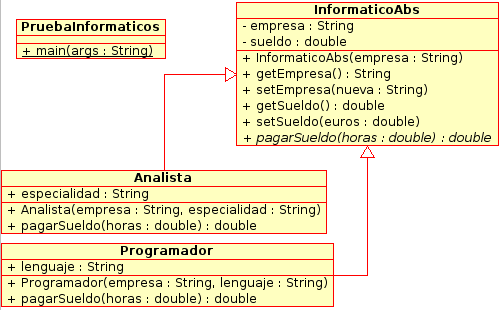
\includegraphics[scale=0.7]{ejercicio1.png}
\\
\vspace*{0.5cm}\\
Implementa las clases especificadas en dicho diagrama, teniendo en cuenta el paradigma de herencia dentro de la POO que ofrece Java.
Comprueba su correcto funcionamiento.

\subsection*{Ejercicio 2}
Dado el siguiente diagrama UML:\\
\vspace*{0.5cm}\\
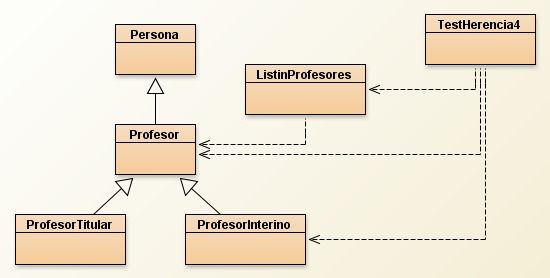
\includegraphics[scale=0.7]{ejercicio2.png}
\\
\vspace*{0.5cm}\\
Trata de definir el c�digo de las clases, estableciendo las relaciones de herencia y uso entre ellas. Trata de crear una clase con el m�todo main (TestHerencia4) donde de alguna manera crees objetos de los distintos tipos y hagas uso de ellos, por ejemplo crea profesores interinos y titulares y luego rec�rrelos con un for extendido donde el tipo sea Profesor. 

\subsection*{Ejercicio 3}
Un videojuego tiene \textbf{Personajes}. Cada personaje tiene un nombre y un nivel propio de energ�a. Adem�s implementan el m�todo alimentarse, que recibe por par�metro una cantidad de energ�a con el que incrementa el nivel propio de energ�a. Los personajes pueden ser:
\begin{description}
\item[Guerreros] tienen adem�s un \emph{arma}. Al momento de la instanciaci�n reciben su \emph{nombre, arma y nivel propio de energ�a inicial}. Los guerreros tienen un m�todo combatir que recibe por par�metro \emph{la cantidad de energ�a} a gastar en el ataque, la cual es descontada de \emph{su nivel propio de energ�a}. El m�todo combatir retorna el \emph{arma} y \emph{la cantidad de energ�a} del ataque concatenados. 
\item[Magos] tienen adem�s un \emph{poder}. Al momento de la instanciaci�n reciben su \emph{nombre} y poder. Los magos son siempre creados con \emph{un nivel propio de energ�a} igual a 100. Proveen un m�todo\emph{encantar}, que disminuye en 2 unidades \emph{el nivel propio de energ�a} y que retorna \emph{el
poder} del mago.
\end{description}
Implementa las clases que consideres oportunas y crea una clase TestVideojuego que compruebe el funcionamiento de las mismas.
\end{document}
